\documentclass[a5paper,12pt]{article}
\usepackage{/../../style}


\newcommand{\montitre}{Logique }


\begin{document}

\fiche{Langage}
\titre{Alphabet} : $\Sigma$ = ensemble de lettres ou symboles. \\

\par

\titre{mot} sur $\Sigma$ = suite finie de lettres \\

\par

\titre{$\Sigma^*$} = tous les mots sur $\Sigma$ \\

\par

\titre{$\epsilon$} = mot vide ($\epsilon \in \Sigma^*$) \\

\par

\titre{Langage} = partie de $\Sigma^*$ (contient ou non $\epsilon$)\\

\par

\titre{Concaténation} : $(\Sigma^*,.)$ est un monoïde libre (loi interne associative avec élément neutre) \\

\par

\titre{Homomorphisme} : $h\ffonc{\Sigma^*}{\Gamma^*}$ tel que : $\left\{ \begin{array}{l} h(\epsilon) = \epsilon \\ h(uv) = h(u)h(v) \end{array} \right.$\\
\par

\titre{Synthaxe} = écriture des mots \\

\par

\titre{Sémantique} = signification des mots 


\fiche{Arbres (déf par les graphes)}
\titre{Arbre libre} : Graphe non orienté connexe et sans circuit \\
\titre{Feuille} = un seul voisin \\
\titre{Etiquette} = $A$ un ensemble et $(V,\Gamma)$ un arbre libre, à chaque élément de $V$ on associe un élément de $A$. \\

\par

\titre{Arbre enraciné} : Arbre libre tel que $\exist r\in V \tq \forall x \in V \exist! c$ chemin entre $x$ et $r$ \\ 
\titre{Arité} d'un sommet = nombre d'enfants \\
\titre{Hauteur} de l'arbre = longueur du plus grand chemin entre la racine et une feuille. \\

\par

\titre{Arbre ordonné} : Arbre dans lequel l'ensemble des enfants de chaque sommet est totalement ordonné. 


\fiche{Induction}
\titre{Définition inductive} : Soit $E$ un ensemble, on définit $X$ le plus petit sous ensemble de $E$ tel que : \\ $ \left\{ \begin{array}{l} (B) : B\subset X \\ (I) : (r_i : \ffonc{E^{n_i}}{E}) \end{array} \right. $ \\
$B$ est la base et $I$ l'ensemble des règles d'induction. \\

\par

\titre{Notations} (exemples) \\
$\N = \left\{ \begin{array}{l} (B) : 0 \in \N \\ (I) : \forall n \in \N, n+1\in \N \end{array} \right.
= \left\{ \frac{}{0} \; \frac{n}{n+1} \right\}$\\
$\Sigma^* = \left\{ \begin{array}{l} (B) : \epsilon \in \Sigma^* \\ (I) : \forall w \in \Sigma^*, a\in\Sigma, wa\in \Sigma^* \end{array} \right. = \left\{ \frac{}{\epsilon} \; \frac{w}{wa} \right\}$ \\
$\{ a^nbc^n \} = \left\{ \frac{}{b} \frac{x}{axc} \right\}$ \\

\par

\titre{Preuve par induction} $\mathcal{P}$ est vraie sur $X$ si et seulement si : \\
$\left\{ \begin{array}{l} \mathcal{P} \; \mathrm{vraie} \; \mathrm{sur} \; B \\ \mathcal{P} \; \mathrm{stable} \; \mathrm{par} \; (I) \end{array} \right.$ \\

\par

\titre{Fonction définie inductivement} : \\
On définit $f$ sur $B$ \\
$\forall x = r_i(x_1,\ldots,x_{n_i})\in X, f(x) = r_i(f(x_1),\ldots,f(x_{n_i}))$ 


\fiche{Arbres (déf par induction)}
\titre{Arbre ordonné} \\
$\left\{ \begin{array}{l}
	\vide \in V \\
	\forall (x_1,\ldots , x_n)  \in X \; \mathrm{liste}\;\mathrm{ordonnee}, \forall v \in V, (v,x_1,\ldots,x_n) \in X
\end{array} \right.$  \\

\par

\titre{Arbre binaire} \\
$\left\{ \begin{array}{l}
	\vide \in A \\
	\forall A_g,A_d \in A, r\in X, (A_g,r,A_d)\in A
\end{array} \right.$ \\

\par

\titre{Arbre binaire étiqueté par un ensemble $A$} \\
$\left\{ \begin{array}{l}
	\vide \in AB \\
	\forall g,d \in AB, \forall a \in A, (g,a,d)\in AB 
\end{array}
\right.$\\

\par

\titre{ATTENTION} Les deux arbres ci-dessous sont les mêmes arbres ordonnés, mais pas les mêmes arbres binaires : \\
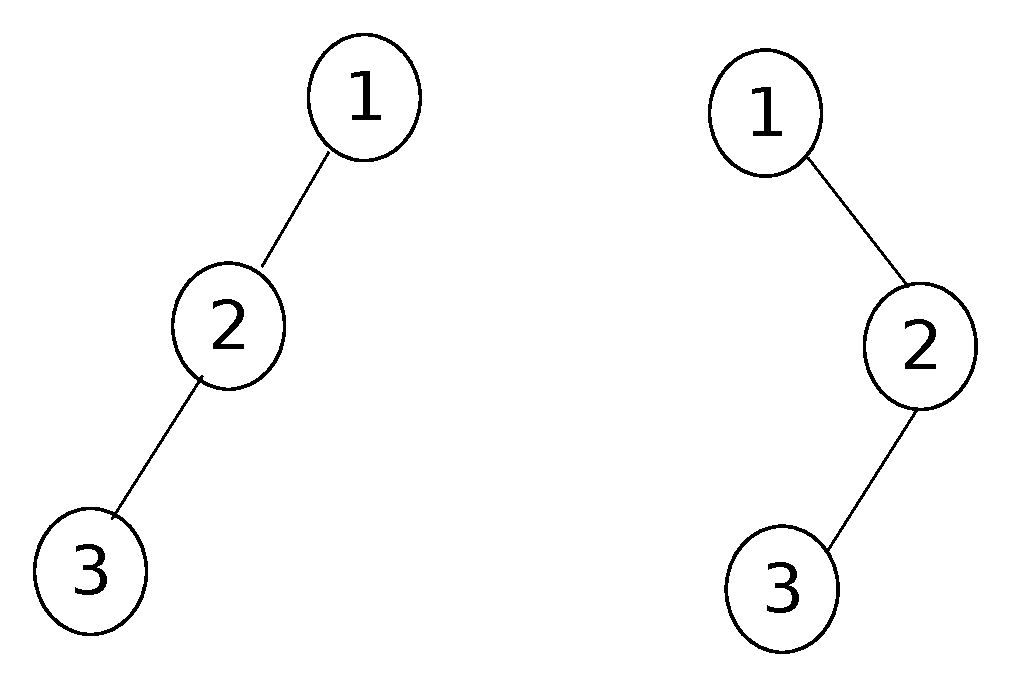
\includegraphics[width=5cm]{D4_1.pdf} \\
Arbre de gauche : $(((\vide,3,\vide),2,\vide),1,\vide)$ \\
Arbre de droite : $(\vide,1,((\vide,3,\vide),2,\vide)$


\fiche{Arbres binaires (déf explicite)}
\titre{Définition par récurrence} : \\
$\left. \begin{array}{l}
	AB_0 =\{\vide\} \\
  AB_{n+1} = AB_n\bigcup \{(g,a,d),a\in A,\;g,d\in AB_n\}
	\end{array}\right\}
AB_{rec}=\displaystyle{\bigcup_{\N}} AB_n$

\titre{Rappel} : \\
$\left\{ \begin{array}{l}
	(B) : \vide \in AB \\
	(I) \forall g,d \in AB, \forall a \in A, (g,a,d)\in AB 
\end{array}
\right.$\\

\titre{Propriété} : $AB_{rec} = AB$

\titre{Preuve} : \begin{enumerate}
\item Montrons que $AB_{rec} \subset AB$, (montrons que $AB_n\subset AB \forall n$) \\
	$AB_0 = \{\vide\} \subset AB$\\
	Supposons $AB_n \subset AB$ et montrons que $AB_{n+1}\subset AB$ \\
	Soit $x\in AB_{n+1} = AB_n\bigcup \{ (g,a,d), a\in A, g,d \in AB_n \}$ \\
	Si $x\in AB_n$ alors $x\in AB$ par hypothèse de récurrence \\
	Sinon $x=(g,a,d)$, $g,d \in AB_n\subset AB$ et $a\in A$ donc $x\in AB$ d'après $(I)$
\item Montrons que $AB\subset AB_{rec}$ (il suffit de montrer que $AB_{rec}$ respecte $(B)$ et $(I)$) \\
	$\vide\in AB_0 \subset AB_{rec}$ donc $AB_{rec}$ vérifie $(B)$.\\
	Soient $g,g\in AB_{req}, \exist p \in \N \tq g,d\in AB_p$ \\
	Donc $\forall a\in A, (g,a,d)\in AB_{p+1}\subset AB_{rec}$ \\
	Donc $AB_{rec}$ respecte $(I)$
\end{enumerate}
	


\fiche{Arbres binaires stricts}
\titre{Définition} \\
$\left\{ \begin{array}{l}
	(B) : (\vide,a\vide)\in ABS \forall a \in A \\
	(I) : \forall g,d\in ABS, \forall a\in A, (g,a,d)\in ABS 
\end{array} \right.$ \\
\par
\titre{Propriété} : $n=2f-1$ ($n=$ nombre de sommets, $f=$ nombre de feuilles) \\
\titre{Preuve} ;
	\begin{enumerate}
	\item Montrons que $\mathcal{P}$ est vraie sur $B$ \\
	Pour $(\vide,a,\vide)$, on a $n=1$ et $f=1$ donc $\mathcal{P}$ vraie ($2\times 1 - 1 = 1$) \\
	\item Supposons $\mathcal{P}$ vraie pour $g$ et $d$ dans $ABS$ et montrons que $\mathcal{P}$ est vraie pour $(g,a,d)$. \\
	$f=f_g+f_d$ et $n=n_g+n_d+1$ \\
	Donc $n=2f_g-1+2f_d-1+1 = 2f-1$
	\end{enumerate}
	


\fiche{Termes}
Soit $F=\{f_0,\ldots,f_n,\ldots\}$ un ensemble de \titre{symboles de fonctions} (prenant un certain nombre d'\titre{arguments}, pas le même nombre pour chaque fonction). \\

Soit $\varphi\ffonc{F}{\N}$ qui à une fonction associe le \titre{nombre d'arguments} qu'elle prend (aussi appelé \titre{arité} de la fonction)\\

\par
\titre{$F_n=\{f\in F \tq \varphi(f)=n\}$} ($F_0 =$ les constantes (on peut donc les utiliser comme arguments des autres fonctions). \\

\par
\titre{Termes} sur $F$ : On définit $T$ inductivement : \\
$\left\{ \begin{array}{l}
	(B) : F_0 \subset T \\
	(I) : \forall t_1,\ldots,t_n\in T, f\in F_n, f(t_1,\ldots,t_n)\in T
\end{array} \right.$

\titre{Lien avec les arbres ordonnés étiquetés par $F$}\\
$F=\{0,1,f,g\}\; F_0=\{0,1\}] \; F_1=\{g\} \; F_2=\{f\}$ \\
Donnons une liste (non exhaustive!) d'éléments de $T$ : \\
$0 \; ; \; 1 \; ; \; g(0) \; ; \; g(1) \; ; \; f(0,1) \; ; \; f(1,0) \; ; \; f(0,g(f(0,1))) \ldots$\\
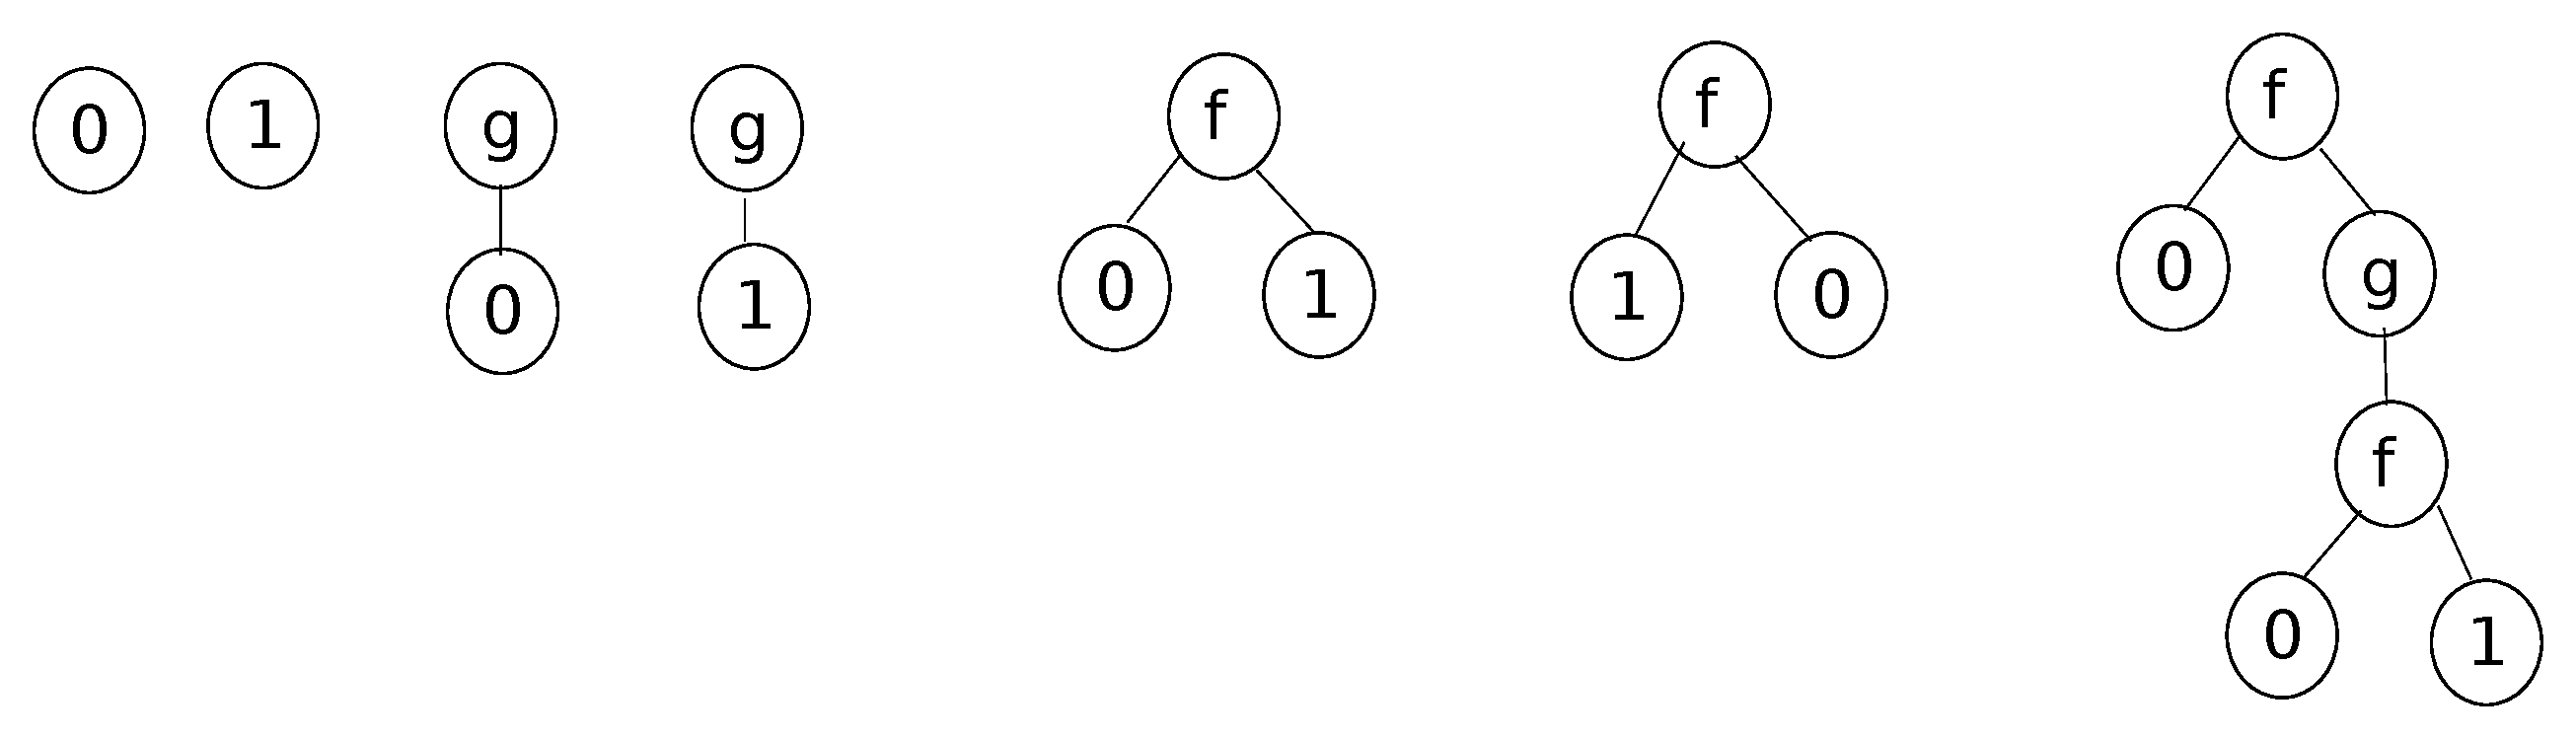
\includegraphics[width=0.8\linewidth]{D7_1.pdf}


\fiche{Dérivation}
Soit $X$ définit \titre{inductivement} par une base $(B)$ et un ensemble de règles $(I)$. On peut aussi définir $X$ par \titre{récurrence} : \\
$\left. \begin{array}{l}
	X_0=B \\
	X_{n+1} = X_n\bigcup \{r_i(x_1,\ldots,x_{n_i}),x_1,\ldots,x_{n_i}\in X_n\}
\end{array} \right\} X=\displaystyle{\bigcup_{\N}}X_n$\\
(pour la preuve, voir l'exemple des arbres binaires définis par récurrence)\\

\par

\titre{Lien avec les termes}\\
$F=B\bigcup I$ ($B=F_0$) \\
\titre{Ensemble des dérivations de $X$} = $D=$ termes sur $F$\\
\par
On pose $h : \begin{array}{lcl}
	D & \longrightarrow & X \\
	b\in B & \longrightarrow & b \\
	r_i(t_1,\ldots,t_{n_i}) & \longrightarrow & r_i(h(t_1),\ldots, h(t_{n_i})) 
\end{array}$\\
\par
La propriété $X=\bigcup X_n$ se réécrit alors \titre{$$X=h(D)=\{h(d),d\in D\}$$} \\

\par
Si $h$ est \titre{injective}, on parle de définition \titre{non ambigüe} (le chemin pour atteindre un élément est unique.


\end{document}
